\begin{figure*}

  \begin{panel}{(a)}{\textwidth}
    \def\histogramcsv{figures/data/sim_counting/intensity_histogram.csv}
    \def\tracecsv{figures/data/sim_counting/trace_and_fit_N10.csv}
    \def\traceintensitycol{trace}
    \def\zcol{fit}
    \def\histbincol{N10_bins}
    \def\histcountcol{N10_measured}
    \def\modelfitcol{N10_model}
    \tikzsetnextfilename{figure_2_trace_N10}
    \begin{tikzpicture}%
  \begin{axis}[
    name=trace,
    width=0.8\textwidth,
    height=5cm,
    xlabel=frames,
    ylabel=intensity,
    enlarge x limits=false,
    xtick distance=500,
    grid=major,
    grid style={dashed},
    scaled ticks=false,
    ticklabel style={font=\small},
    legend style={nodes={scale=0.6, transform shape}},
  ]

    \addplot [
      color=tracecolor,
      mark=*,
      mark size=0.7pt,
      mark options={line width=0},
      fill opacity=0.8,
      draw opacity=0.2,
    ] table [
      col sep=comma,
      x=frames,
      y=\traceintensitycol
    ] {\tracecsv};
    \addlegendentry{intensity trace}

    \addplot [
      color=ztracecolor,
      thick
    ] table [
      col sep=comma,
      x=frames,
      y=\zcol
    ] {\tracecsv};
    \addlegendentry{inferred state}

    % remember min/max y-axis values for next plot
    \pgfplotsextra{
      \pgfmathparse{\pgfkeysvalueof{/pgfplots/ymin}}
      \global\let\ymin\pgfmathresult
      \pgfmathparse{\pgfkeysvalueof{/pgfplots/ymax}}
      \global\let\ymax\pgfmathresult
    }

  \end{axis}

  \begin{axis}[
    at={($(trace.east) + (4mm,0)$)},
    anchor=west,
    width=0.3\textwidth,
    height=5cm,
    yticklabel=\empty,
    xtick distance=0.005,
    xlabel=probability,
    grid=major,
    grid style={dashed, very thin},
    enlarge x limits={value=0.1,upper},
    scaled ticks=false,
    ymin=\ymin,
    ymax=\ymax,
    ticklabel style={font=\small},
    legend style={nodes={scale=0.6, transform shape}},
  ]

    \addplot+[
      xbar interval,
      mark=none,
      color=tracecolor,
      fill=tracecolor,
      fill opacity=0.6,
      draw=none,
    ] table [
      col sep=comma,
      y=\histbincol,
      x=\histcountcol,
    ] {\histogramcsv};
    \addlegendentry{intensity histogram}

    \addplot[
      color=intensitymodelcolor!80!black,
      thick
    ] table [
      col sep=comma,
      y=\histbincol,
      x=\modelfitcol
    ] {\histogramcsv};
    \addlegendentry{inferred model}

  \end{axis}
\end{tikzpicture}%
%
  \end{panel}

  \begin{panel}{(b)}{\textwidth}
    \def\histogramcsv{figures/data/sim_counting/intensity_histogram.csv}
    \def\tracecsv{figures/data/sim_counting/trace_and_fit_N20.csv}
    \def\traceintensitycol{trace}
    \def\zcol{fit}
    \def\histbincol{N20_bins}
    \def\histcountcol{N20_measured}
    \def\modelfitcol{N20_model}
    \tikzsetnextfilename{figure_2_trace_N20}
    \begin{tikzpicture}%
  \begin{axis}[
    name=trace,
    width=0.8\textwidth,
    height=5cm,
    xlabel=frames,
    ylabel=intensity,
    enlarge x limits=false,
    xtick distance=500,
    grid=major,
    grid style={dashed},
    scaled ticks=false,
    ticklabel style={font=\small},
    legend style={nodes={scale=0.6, transform shape}},
  ]

    \addplot [
      color=tracecolor,
      mark=*,
      mark size=0.7pt,
      mark options={line width=0},
      fill opacity=0.8,
      draw opacity=0.2,
    ] table [
      col sep=comma,
      x=frames,
      y=\traceintensitycol
    ] {\tracecsv};
    \addlegendentry{intensity trace}

    \addplot [
      color=ztracecolor,
      thick
    ] table [
      col sep=comma,
      x=frames,
      y=\zcol
    ] {\tracecsv};
    \addlegendentry{inferred state}

    % remember min/max y-axis values for next plot
    \pgfplotsextra{
      \pgfmathparse{\pgfkeysvalueof{/pgfplots/ymin}}
      \global\let\ymin\pgfmathresult
      \pgfmathparse{\pgfkeysvalueof{/pgfplots/ymax}}
      \global\let\ymax\pgfmathresult
    }

  \end{axis}

  \begin{axis}[
    at={($(trace.east) + (4mm,0)$)},
    anchor=west,
    width=0.3\textwidth,
    height=5cm,
    yticklabel=\empty,
    xtick distance=0.005,
    xlabel=probability,
    grid=major,
    grid style={dashed, very thin},
    enlarge x limits={value=0.1,upper},
    scaled ticks=false,
    ymin=\ymin,
    ymax=\ymax,
    ticklabel style={font=\small},
    legend style={nodes={scale=0.6, transform shape}},
  ]

    \addplot+[
      xbar interval,
      mark=none,
      color=tracecolor,
      fill=tracecolor,
      fill opacity=0.6,
      draw=none,
    ] table [
      col sep=comma,
      y=\histbincol,
      x=\histcountcol,
    ] {\histogramcsv};
    \addlegendentry{intensity histogram}

    \addplot[
      color=intensitymodelcolor!80!black,
      thick
    ] table [
      col sep=comma,
      y=\histbincol,
      x=\modelfitcol
    ] {\histogramcsv};
    \addlegendentry{inferred model}

  \end{axis}
\end{tikzpicture}%

  \end{panel}

  \vspace{4mm}
  \begin{panel}{(c)}{0.4\textwidth}
    \def\posteriormatrixcsv{figures/data/sim_counting/heatmap.csv}
    \def\lbfcscsv{figures/data/sim_counting/heatmap_lbfcs.csv}
    \tikzsetnextfilename{figure_2_lbfcs_comparison}
    \begin{tikzpicture}
  \begin{axis}[
    name=trace,
    width=\textwidth,
    height=\textwidth,
    xlabel=Estimated \n,
    ylabel=True \n,
    enlarge x limits=false,
    enlarge y limits=false,
    grid=major,
    grid style={dashed},
    scaled ticks=false,
    ticklabel style={font=\small},
    xtick align=outside,
    xtick pos=lower,
    ytick align=outside,
    ytick pos=lower,
    colorbar,
  ]

    \pgfplotsset{
      colormap={posteriorcolormap}{
        color(0.0)=(white)
        color(0.2)=(funkey_color_2)
        color(1.0)=(funkey_color_2!50!black)
      }
    }

    \addplot[
      matrix plot*,
      mesh/cols=35,
      point meta=explicit,
    ] table [
      col sep=comma,
      x=n,
      y=true_n,
      meta=posterior,
    ] {\posteriormatrixcsv};

  \end{axis}

  \begin{axis}[
    name=trace,
    width=\textwidth,
    height=\textwidth,
    xmin=0.5,
    xmax=35.5,
    ymin=0.5,
    ymax=30.5,
    grid=major,
    grid style={dashed},
    scaled ticks=false,
    domain=0:35,
    ticklabel style={font=\small},
  ]

    \addplot[
      mark=*,
      only marks,
      mark size=1.4pt,
      mark options={draw=white,fill=funkey_color_1,draw opacity=0.6,fill opacity=0.7},
    ] table [
      col sep=comma,
      x=lbfcs_count,
      y=n,
    ] {\lbfcscsv};

    \addplot[no marks,thick,gray] {x};

  \end{axis}

\end{tikzpicture}

  \end{panel}
  \hspace{1cm}
  \begin{panel}{(d)}{0.2\textwidth}
    \def\posteriorcsv{figures/data/sim_counting/posteriors.csv}
    \def\posteriorcol{posterior_10}
    \def\posteriorcolextra{posterior_20}
    \tikzsetnextfilename{figure_2_posterior_n10_n20}
    \@ifundefined{noylabels}{}{%
  \pgfplotsset{yticklabel=\empty}%
}%
\begin{tikzpicture}%

  \def\eps{0.001}

  \begin{axis}[
    width=\textwidth,
    height=\textwidth,
    xlabel=\n,
    xlabel=$p(\n|\trace)$,
    grid=major,
    grid style={dashed, very thin},
    enlarge x limits=0.1,
    enlarge y limits=0,
    ymin=0,
    ymax=1,
    scaled ticks=false,
    ticklabel style={font=\small},
  ]

    \addplot+[
      ybar,
      bar width=1,
      mark=none,
      fill=posteriorcolor,
      fill opacity=0.6,
      draw=posteriorcolor,
      y filter/.expression={
        y < \eps ? nan : y
      },
    ] table [
      col sep=comma,
      y=\posteriorcol,
      x=n,
    ] {\posteriorcsv};

    \ifdefined\posteriorcolextra
      \addplot+[
        ybar,
        bar width=1,
        mark=none,
        fill=posteriorcolor!60!black,
        fill opacity=0.6,
        draw=posteriorcolor,
        y filter/.expression={
          y < \eps ? nan : y
        },
      ] table [
        col sep=comma,
        y=\posteriorcolextra,
        x=n,
      ] {\posteriorcsv};
    \fi

  \end{axis}

\end{tikzpicture}

  \end{panel}
  \begin{panel}{(e)}{0.4\textwidth}
    \def\tracelengthcsv{figures/data/trace_length/trace_length_results.csv}
    \def\mapcol{max_likelihoods_20}
    \def\varcol{variance_20}
    \tikzsetnextfilename{figure_2_trace_length}
    \def\intervalplot#1#2{%
  \addplot[%
    color=#2,%
    very thick,%
  ] table [%
    col sep=comma,%
    x=length,%
    y=max_likelihoods_#1,%
  ] {\tracelengthcsv};%
  \addplot[%
    name path=lower,%
    draw=none,%
    fill=none,%
    forget plot,%
  ] table [%
    col sep=comma,%
    x=length,%
    y expr=\thisrow{max_likelihoods_#1} - \thisrow{variance_#1}%
  ] {\tracelengthcsv};%
  \addplot[%
    name path=upper,%
    draw=none,%
    fill=none,%
    forget plot,%
  ] table [%
    col sep=comma,%
    x=length,%
    y expr=\thisrow{max_likelihoods_#1} + \thisrow{variance_#1}%
  ] {\tracelengthcsv};%
  \addplot [%
    color=#2,%
    opacity=0.4,%
    forget plot,%
  ] fill between[of=lower and upper];%
  \addlegendentry{$n=#1$};
}%
\begin{tikzpicture}
  \begin{axis}[
    width=\textwidth,
    height=0.47\textwidth,
    xlabel={length [frames]},
    %ylabel=estimated count,
    enlarge x limits=false,
    enlarge y limits=false,
    xtick distance=4000,
    ytick distance=5,
    ymin=0,
    grid=major,
    grid style={dashed},
    scaled ticks=false,
    ticklabel style={font=\small},
    legend columns=4,
    legend style={nodes={scale=0.6, transform shape}},
  ]
    \intervalplot{20}{funkey_color_1}
    \intervalplot{15}{funkey_color_2}
    \intervalplot{10}{funkey_color_3}
    \intervalplot{5}{funkey_color_4}
  \end{axis}
\end{tikzpicture}%

  \end{panel}

\end{figure*}


\begin{figure*}
  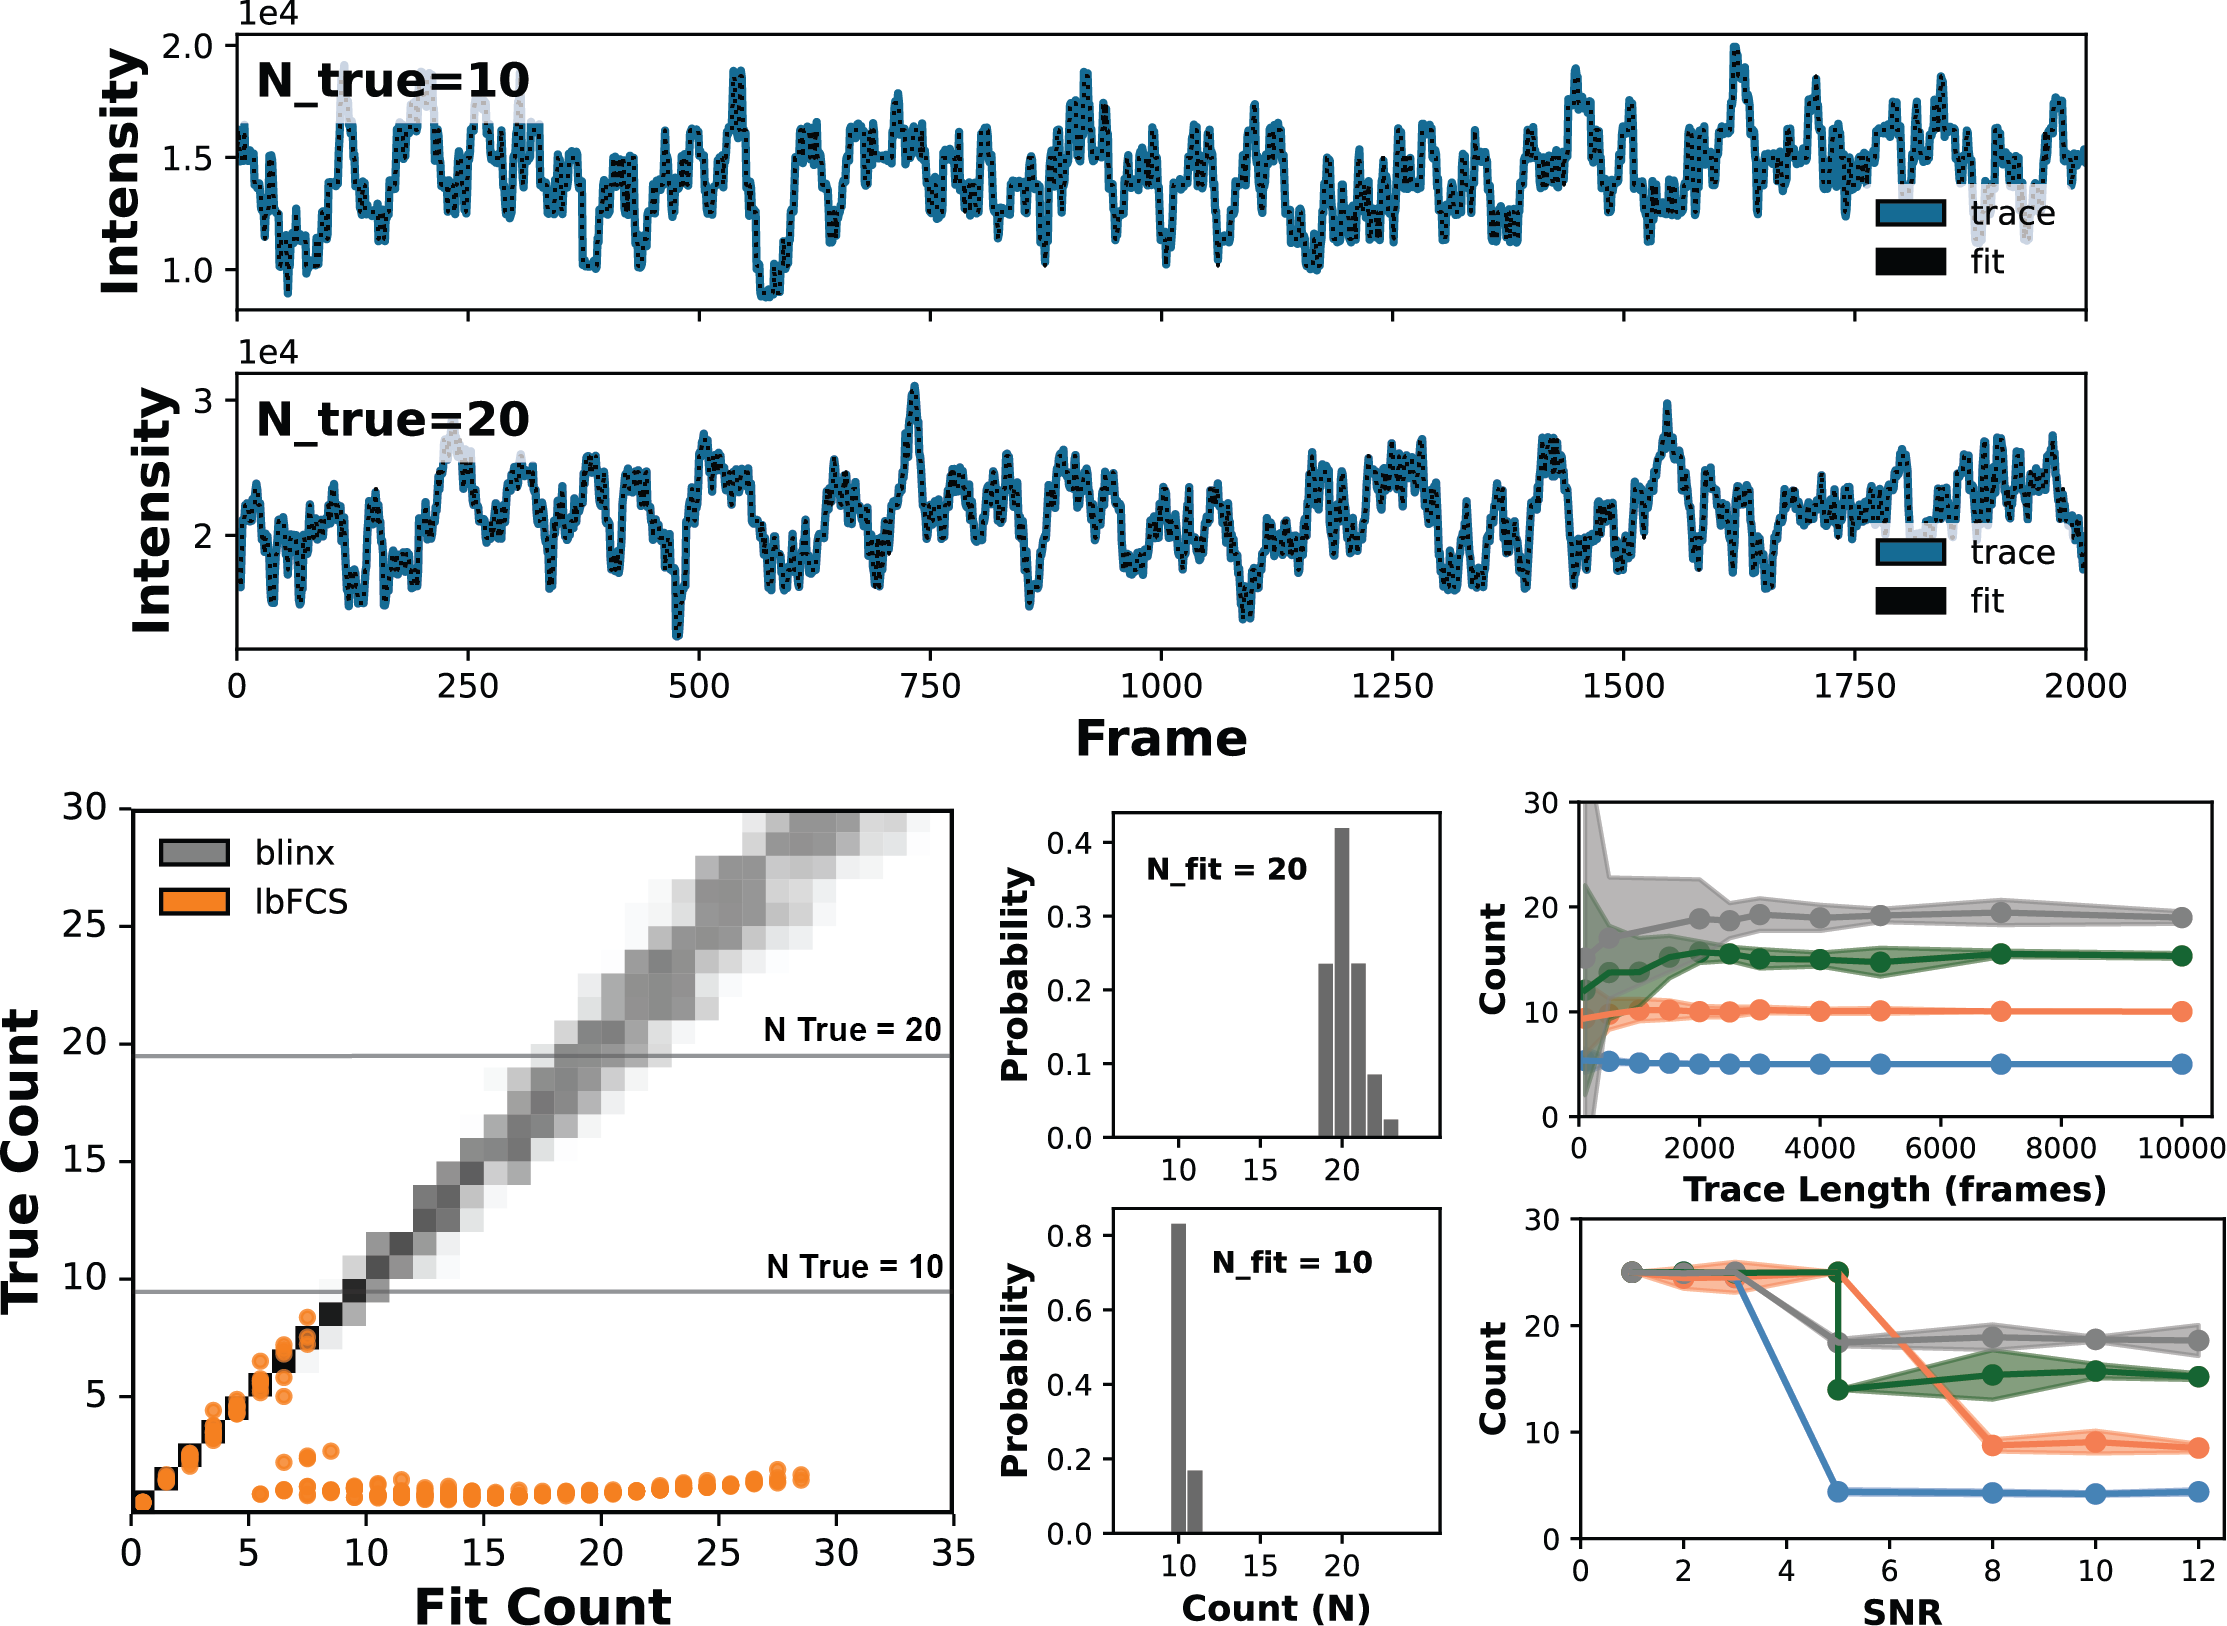
\includegraphics[width=\linewidth]{figures/placeholders/figure_2_simulated_counting.png}
  \caption{A) Trace simulated from 10 emitters, and the posterior distribution estimated by blinx B) simulated from 20 emitters
  C) The blinx posterior is able to accurately estimate significantly higher molecular counts than the current state of the art, lbFCS
  D) As trace length increases, the variance of the blinx posterior decreases E) As the signal to noise ratio increases the variance of 
  the blinx posterior decreases. }
  \label{fig:method:overview}
\end{figure*}
